\begin{figure}[ht]
\centering
% Reuse Nature CNN colors
\definecolor{convfront}{HTML}{7BA4CC}
\definecolor{convtop}{HTML}{9CBDDD}
\definecolor{convside}{HTML}{5A87B5}
\definecolor{fcfront}{HTML}{B3CEE4}
\definecolor{fctop}{HTML}{CDDEF0}
\definecolor{fcside}{HTML}{8DB3D2}
\definecolor{outfront}{HTML}{DCE8F4}
\definecolor{outtop}{HTML}{EBF1F8}
\definecolor{outside}{HTML}{C2D6E8}
% Probe colors
\definecolor{probeorange}{HTML}{E8B87A}
\definecolor{predorange}{HTML}{F5E0C8}
\definecolor{gtgreen}{HTML}{D4ECD4}
% Faded encoder
\definecolor{encfade}{HTML}{B8D2E6}

%% --- (a) Frozen encoder concept ---
\begin{subfigure}[t]{\textwidth}
\centering
\resizebox{0.92\textwidth}{!}{%
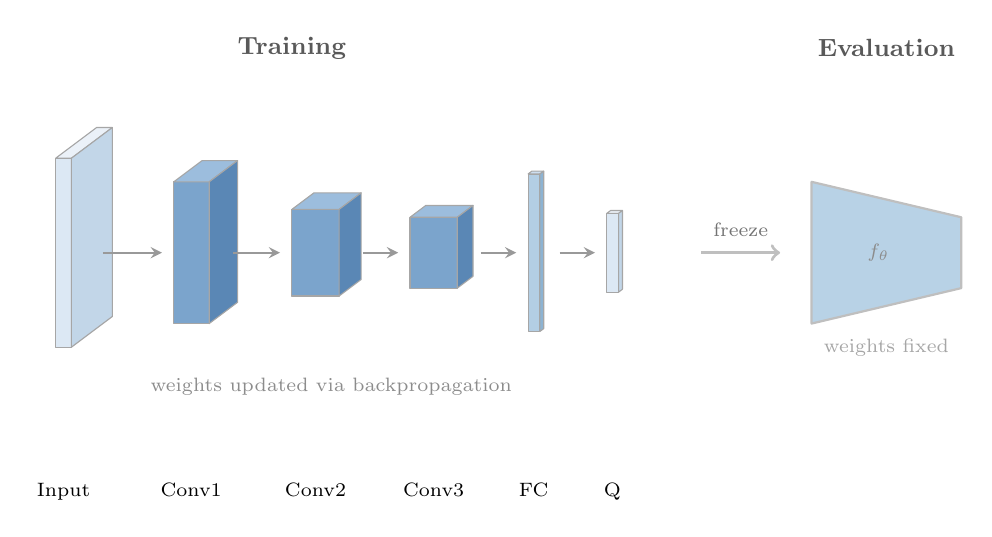
\begin{tikzpicture}[
    x={(1cm,0cm)}, y={(0cm,1cm)}, z={(0.4cm,0.3cm)},
    arr/.style={->, thick, >=stealth, black!40},
    lbl/.style={font=\scriptsize, text=black!55},
    phase/.style={font=\small\bfseries, text=black!65},
    namelbl/.style={font=\scriptsize, anchor=north},
]

\newcommand{\cuboid}[7]{
    \fill[#5, draw=black!35, line join=round]
        (#1, {-#3/2}, 0) -- ({#1+#2}, {-#3/2}, 0) --
        ({#1+#2}, {#3/2}, 0) -- (#1, {#3/2}, 0) -- cycle;
    \fill[#6, draw=black!35, line join=round]
        (#1, {#3/2}, 0) -- ({#1+#2}, {#3/2}, 0) --
        ({#1+#2}, {#3/2}, #4) -- (#1, {#3/2}, #4) -- cycle;
    \fill[#7, draw=black!35, line join=round]
        ({#1+#2}, {-#3/2}, 0) -- ({#1+#2}, {#3/2}, 0) --
        ({#1+#2}, {#3/2}, #4) -- ({#1+#2}, {-#3/2}, #4) -- cycle;
}

\def\dimY{-2.8}

% Phase label
\node[phase] at (3.0, 2.6) {Training};

% Input
\cuboid{0}{0.2}{2.4}{1.3}{outfront}{outtop}{outside}
\node[namelbl] at (0.1, \dimY) {Input};

\draw[arr] (0.6, 0, 0) -- (1.35, 0, 0);

% Conv1
\cuboid{1.5}{0.45}{1.8}{0.9}{convfront}{convtop}{convside}
\node[namelbl] at (1.72, \dimY) {Conv1};

\draw[arr] (2.25, 0, 0) -- (2.85, 0, 0);

% Conv2
\cuboid{3.0}{0.6}{1.1}{0.7}{convfront}{convtop}{convside}
\node[namelbl] at (3.3, \dimY) {Conv2};

\draw[arr] (3.9, 0, 0) -- (4.35, 0, 0);

% Conv3
\cuboid{4.5}{0.6}{0.9}{0.5}{convfront}{convtop}{convside}
\node[namelbl] at (4.8, \dimY) {Conv3};

\draw[arr] (5.4, 0, 0) -- (5.85, 0, 0);

% FC
\cuboid{6.0}{0.15}{2.0}{0.12}{fcfront}{fctop}{fcside}
\node[namelbl] at (6.07, \dimY) {FC};

\draw[arr] (6.4, 0, 0) -- (6.85, 0, 0);

% Q-head
\cuboid{7.0}{0.15}{1.0}{0.12}{outfront}{outtop}{outside}
\node[namelbl] at (7.07, \dimY) {Q};

% Trainable label
\node[font=\scriptsize, text=black!45] at (3.5, -1.7, 0)
    {weights updated via backpropagation};

% --- Freeze arrow ---
\draw[->, very thick, black!25]
    (8.2, 0) -- (9.2, 0)
    node[midway, above=2pt, lbl] {freeze};

% --- Phase 2: Frozen encoder (compact trapezoid) ---
\node[phase] at (10.55, 2.6) {Evaluation};

% Compact encoder trapezoid (no inputs/outputs -- (b) covers that)
\fill[encfade, draw=black!25, thick, line join=round]
    (9.6, -0.9) -- (9.6, 0.9) -- (11.5, 0.45) -- (11.5, -0.45) -- cycle;
\node[font=\scriptsize, text=black!45] at (10.45, 0) {$f_\theta$};

\node[lbl, text=black!35] at (10.55, -1.2) {weights fixed};

\end{tikzpicture}%
}
\caption{The encoder is trained end-to-end via RL, then its weights
  are frozen for linear probing.}
\label{fig:frozen-encoder}
\end{subfigure}

\vspace{1.2em}

%% --- (b) Linear probe concept ---
\begin{subfigure}[t]{\textwidth}
\centering
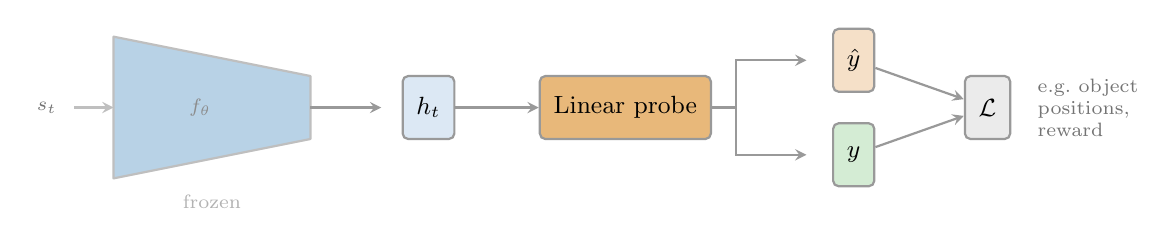
\begin{tikzpicture}[
    box/.style={draw=black!40, thick, minimum height=0.8cm,
                font=\small, inner sep=5pt, rounded corners=2pt},
    arr/.style={->, thick, >=stealth, black!40},
    lbl/.style={font=\scriptsize, text=black!55},
]

% Frozen encoder (trapezoid matching subfigure a)
\node[lbl] at (-0.1, 0) [left] {$s_t$};
\draw[arr, black!25] (0.0, 0) -- (0.5, 0);

\fill[encfade, draw=black!25, thick, line join=round]
    (0.5, -0.9) -- (0.5, 0.9) -- (3.0, 0.4) -- (3.0, -0.4) -- cycle;
\node[font=\scriptsize, text=black!45] at (1.6, 0) {$f_\theta$};
\node[lbl, text=black!30] at (1.75, -1.2) {frozen};

% h_t
\draw[arr] (3.0, 0) -- (3.9, 0);
\node[box, fill=outfront] (repr) at (4.5, 0) {$h_t$};

% Linear probe
\draw[arr] (repr) -- (5.9, 0);
\node[box, fill=probeorange, minimum width=1.6cm] (probe)
    at (7.0, 0) {Linear probe};

% Fork to prediction and ground truth
\draw[arr] (probe.east) -- ++(0.3,0) |- (9.3, 0.6);
\draw[arr] (probe.east) -- ++(0.3,0) |- (9.3, -0.6);

\node[box, fill=predorange] (pred) at (9.9, 0.6) {$\hat{y}$};
\node[box, fill=gtgreen] (gt) at (9.9, -0.6) {$y$};

% Loss
\node[box, fill=black!8, font=\small] (loss) at (11.6, 0)
    {$\mathcal{L}$};
\draw[arr] (pred) -- (loss);
\draw[arr] (gt) -- (loss);

% Annotation
\node[lbl, anchor=west, align=left] at (loss.east) [xshift=6pt]
    {e.g.\ object\\positions,\\reward};

\end{tikzpicture}
\caption{A linear probe is trained on frozen representations to
  predict game-state properties. Probe accuracy measures what
  information $h_t$ contains.}
\label{fig:linear-probe-concept}
\end{subfigure}

\vspace{1.2em}

%% --- (c) Probe attachment points ---
\begin{subfigure}[t]{\textwidth}
\centering
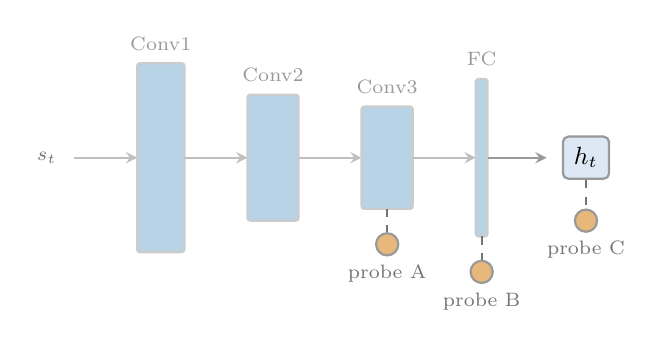
\begin{tikzpicture}[
    arr/.style={->, thick, >=stealth, black!40},
    lbl/.style={font=\scriptsize, text=black!55},
    blklbl/.style={font=\scriptsize, text=black!40},
    probemark/.style={circle, fill=probeorange, draw=black!40,
                      thick, minimum size=8pt, inner sep=0pt},
]

% Input
\node[lbl] at (-0.1, 0) [left] {$s_t$};
\draw[arr, black!25] (0.0, 0) -- (0.8, 0);

% Conv1
\fill[encfade, draw=black!20, thick, rounded corners=1pt]
    (0.8, -1.2) rectangle (1.4, 1.2);
\node[blklbl] at (1.1, 1.45) {Conv1};

\draw[arr, black!25] (1.4, 0) -- (2.2, 0);

% Conv2
\fill[encfade, draw=black!20, thick, rounded corners=1pt]
    (2.2, -0.8) rectangle (2.85, 0.8);
\node[blklbl] at (2.525, 1.05) {Conv2};

\draw[arr, black!25] (2.85, 0) -- (3.65, 0);

% Conv3
\fill[encfade, draw=black!20, thick, rounded corners=1pt]
    (3.65, -0.65) rectangle (4.3, 0.65);
\node[blklbl] at (3.975, 0.9) {Conv3};

\draw[arr, black!25] (4.3, 0) -- (5.1, 0);

% FC
\fill[encfade, draw=black!20, thick, rounded corners=1pt]
    (5.1, -1.0) rectangle (5.25, 1.0);
\node[blklbl] at (5.175, 1.25) {FC};

\draw[arr] (5.25, 0) -- (6.0, 0);

% h_t
\node[draw=black!40, thick, fill=outfront, rounded corners=2pt,
      font=\small, inner sep=4pt] (ht) at (6.5, 0) {$h_t$};

% Probe markers
\node[probemark] (m3) at (3.975, -1.1) {};
\node[probemark] (mfc) at (5.175, -1.45) {};
\node[probemark] (mr) at (6.5, -0.8) {};

\draw[thick, dashed, black!55] (3.975, -0.65) -- (m3);
\draw[thick, dashed, black!55] (5.175, -1.0) -- (mfc);
\draw[thick, dashed, black!55] (ht.south) -- (mr);

\node[lbl] at (m3) [below=4pt] {probe A};
\node[lbl] at (mfc) [below=4pt] {probe B};
\node[lbl] at (mr) [below=4pt] {probe C};

\end{tikzpicture}
\caption{Independent probes at different depths reveal how
  information develops through the network
  (see \cref{fig:nature-cnn} for architecture details).}
\label{fig:linear-probe-layers}
\end{subfigure}

\caption{Linear probe methodology. (a)~The encoder trains via RL and
  is then frozen. (b)~A linear probe predicts game-state properties
  from the frozen encoder's representations. (c)~Probes attached at
  multiple layers measure how information develops across the network.}
\label{fig:linear-probe}
\end{figure}
